%\documentclass[12pt,a4paper,english]{article}%
\RequirePackage[l2tabu, orthodox]{nag}
\documentclass[11pt,a4paper,english]{amsart}
%%%%%%%%%%%%% %%%%%%%%%%%%% %%%%%%%%%%%%% %%%%%%%%%
%%%%%%%%%%%%% MATH %%%%%%%%
%%%%%%%%%%%%% %%%%%%%%%%%%% %%%%%%%%%%%%% %%%%%%%%
\usepackage{amssymb}
\usepackage{amsfonts}
\usepackage{amsmath}
\usepackage{mathrsfs}


%%%%%%%%%%%%% %%%%%%%%%%%%% %%%%%%%%%%%%% %%%%%%%%%
%%%%%%%%%%%%% TEXT %%%%%%%%
%%%%%%%%%%%%% %%%%%%%%%%%%% %%%%%%%%%%%%% %%%%%%%%
%\usepackage[singlespacing]{setspace}
\usepackage{appendix} %Create a section of appendix
\usepackage{epigraph} % To include epigraph at the begging 
\usepackage{multimedia}
%%%%%%%%%%%%% %%%%%%%%%%%%% %%%%%%%%%%%%% %%%%%%%%%
%%%%%%%%%%%%% MARGINS  %%%%%%%%
%%%%%%%%%%%%% %%%%%%%%%%%%% %%%%%%%%%%%%% %%%%%%%%%%%
% allows for temporary adjustment of side margins
\usepackage{chngpage}
\usepackage[nohead]{geometry}
\geometry{left=1in,right=1in,top=1.00in,bottom=1.0in} 
\usepackage{tikz}

%%%%%%%%%%%%% %%%%%%%%%%%%% %%%%%%%%%%%%% %%%%%%%%%
%%%%%%%%%%%%% DATES %%%%%%%%
%%%%%%%%%%%%% %%%%%%%%%%%%% %%%%%%%%%%%%% %%%%%%%%%%%%
% To put only the month and year in the date.
\usepackage{datetime}


%%%%%%%%%%%%% %%%%%%%%%%%%% %%%%%%%%%%%%% %%%%%%%%%
%%%%%%%%%%%%% LANGUAGES  %%%%%%%%
%%%%%%%%%%%%% %%%%%%%%%%%%% %%%%%%%%%%%%% %%%%%%%%%%%
\usepackage[english]{babel} % Package to set up language
\addto\captionsenglish{
\def\figurename{Graph}
}


%%%%%%%%%%%%% %%%%%%%%%%%%% %%%%%%%%%%%%% %%%%%%%%%
%%%%%%%%%%%%% PACKAGES  FOR TABLES AND FIGURES %%%%%%%%
%%%%%%%%%%%%% %%%%%%%%%%%%% %%%%%%%%%%%%% %%%%%%%%%%%%
\usepackage{graphicx}
\usepackage[capposition=top,facing=yes]{floatrow} % Position and everything with 
\DeclareFloatFont{tiny}{\tiny}% "scriptsize" is defined by floatrow, "tiny" not
\floatsetup[table]{font=tiny}
%\usepackage{lscape}
\usepackage{pdflscape} % Use landscape enviroment, roting the page in PDF.


\usepackage{longtable} % Allow to break tables in two
\usepackage{rotating} % Allow to put tables horizontally
%\usepackage{threeparttable} % Allow to put notes in the tables
\usepackage{ctable} %% Align decimals
\usepackage{booktabs} % just makes the table prettier (see \toprule, \bottomrule, etc. commands below)
\usepackage{multirow} % Multi-row enviroments

\usepackage{arydshln} % Allow to dashed line in tables
\usepackage{tabularx} % Replace tabular NICER

%%%%%%%%%%%%% %%%%%%%%%%%%% %%%%%%%%%%%%% %%%%%%%%%
%%%%%%%%%%%%% REFERENCE - BIBTEX  %%%%%%%%
%%%%%%%%%%%%% %%%%%%%%%%%%% %%%%%%%%%%%%% %%%%%%%%%%%
\usepackage{apacite} % Style of referencing
\usepackage{endnotes} % To put all the footnote at the end
%\usepackage[colorlinks=true,citecolor=black,linkcolor=black,urlcolor=black]{hyperref} % Hyperlinks


%%%%%%%%%%%%% %%%%%%%%%%%%% %%%%%%%%%%%%% %%%%%%%%%
%%%%%%%%%%%%% Others %%%%%%%%
%%%%%%%%%%%%% %%%%%%%%%%%%% %%%%%%%%%%%%% %%%%%%%%%%%

% Commands for reference the table
\newcommand{\goestable}[1]{\begin{center}[Table \ref{table_#1} goes about here]\end{center}}
\newcommand{\goesmap}[1]{\begin{center}[Map \ref{map_#1} goes about here]\end{center}}
\renewcommand{\thefootnote}{\fnsymbol{footnote}}



%%% Generate the code \sym for regression
\def\sym#1{\ifmmode^{#1}\else\(^{#1}\)\fi}


%%% SET UP INPUT FOLDER
\makeatletter

\newif\ifBreak
\Breakfalse

\gdef\inputpaths#1{\gdef\@inputpaths{#1}}
\gdef\@inputpaths{}

\newcommand{\forAllInputpaths}[2][\path]{\@for#1:=\@inputpaths\do{#2}}

\gdef\printinputpaths{
    \forAllInputpaths[\path]{Path: \path}
}



%{{{ redefine include
\global\let\old@include\include
\gdef\includex#1{
    \IfFileExists{#1.tex}
    {
        \old@include{#1}
    }
    {
        \forAllInputpaths[\path]
        {
            \ifBreak
            \else
                \IfFileExists{\path/#1.tex}
                {
                    \old@include{\path/#1}
                    \Breaktrue
                }
                {}
            \fi
        }
        \ifBreak
        \else 
            % \PackageError{includex}{'#1' can not be resolved}{'#1' can not be resolved. It is not in \@includepaths}
            \old@include{#1}
        \fi
        \Breakfalse
    }
}
\gdef\include#1{\includex{#1}}
%}}}
%{{{ redefine input
% original definition of input: \def\input{\@ifnextchar\bgroup\@iinput\@@input}
\global\let\old@input\@@input
\gdef\@@input#1{\old@input#1}
\gdef\inputx#1{
      \IfFileExists{#1.tex}
      {
          \@@input{#1}%
      }
    {
        \forAllInputpaths[\path]
        {
            \ifBreak
            \else
                \IfFileExists{\path/#1.tex}
                {
                    \@@input{\path/#1}
                    \Breaktrue
                }
                {}
            \fi
        }
        \ifBreak
        \else 
            %\PackageError{includex}{'#1' can not be resolved}{'#1' can not be resolved. It is not in \@includepaths}
            \@@input{#1}
        \fi
        \Breakfalse
    }
}
\def\input{\@ifnextchar\bgroup\inputx\@@input}
%}}}
\makeatother



\begin{document}
%<*mytag>
\inputpaths{/Users/jcmunozmora/Documents/data/Tobon-Munoz-Dagust/tables/}
\graphicspath{{maps/}{/Users/jcmunozmora/Documents/data/Tobon-Munoz-Dagust/figures/}}

\section*{Tables and Figures}


%%%%%%%%%%%%%%%%%%%%%%%%%%%%%% 	
%%% TABLE 1 - Summary statistics
%%%%%%%%%%%%%%%%%%%%%%%%%%%%%% 	

\begin{adjustwidth}{-6in}{-6in}% adjust the L and R margins by 1 inch
\begin{centering}
  \begin{table}[H]
\centering
\caption{Overall mean by year for time-varying variables }
\label{table_1} 
\makebox[\textwidth]{%
\setlength{\tabcolsep}{2pt}
\begin{tabularx}{\linewidth}{ X c c c c c c c c c c }
 \hline 
 \input{table_1}\\[-2ex] 
\multicolumn{11}{l}{ \emph{Notes - } Standard errors in brackets. We present the mean over all municipalities each year. Data source: CEDE, 2012.}
\end{tabularx}}
\end{table}
\end{centering}
\end{adjustwidth}


%%%%%%%%%%%%%%%%%%%%%%%%%%%%%% 	
%% TABLE 2 - Mean test 
%%%%%%%%%%%%%%%%%%%%%%%%%%%%%% 

\begin{adjustwidth}{-6in}{-6in}% adjust the L and R margins by 1 inch
\begin{centering}
\begin{table}[H]
 \centering
\caption{Mean test for the time-variant variable by presence of coca 
\label{table_2}
}
\makebox[\textwidth]{%
\begin{tabularx}{\textwidth}{ X c c c}
%\begin{tabular}{p{6cm}p{2cm}p{2cm}p{2cm}} 
\hline
 \input{table_2} \\[-2ex] \hline \multicolumn{4}{p{\linewidth}}{ \emph{Notes - } Standard errors in brackets. Number of observation in the third row. \sym{*} Significant at 10\%, \sym{**} significant at 5\%, and \sym{***} significant at 1\%. Two-side mean test significance reported.  We define presence of coca if a given municipality had at least one year coca. Data source: CEDE, 2012.}
%\end{tabular}
\end{tabularx}
}
\end{table}
\end{centering}
\end{adjustwidth}



%%%%%%%%%%%%%%%%%%%%%%%%%%%%%% 
%% TABLE 3 - Summary time-variant
%%%%%%%%%%%%%%%%%%%%%%%%%%%%%% 

\begin{adjustwidth}{-6in}{-6in}% adjust the L and R margins by 1 inch
\begin{centering}
\begin{table}[H]
 \centering
\caption{Summary statistics for time-variant variables }
\label{table_3}
\makebox[\textwidth]{%
\begin{tabularx}{\linewidth}{ c c c c c c c } \hline
 \input{table_3} \\ \hline
\multicolumn{7}{p{\linewidth}}{ \emph{Notes - } The table reports between and within variations for all time-varying variables. The within transformation demeans the data by subtracting the mean for each municipality and then adding up the overall mean. This explains the negative minimums for positive variables. The \emph{overall observations} are the total number of observations, \emph{between observations} is the number of observations per time period and \emph{within observations} is the number of time periods in which there is data available for each variable.. Data source: CEDE, 2012.}
\end{tabularx}
}
\end{table}
\end{centering}
\end{adjustwidth}

%%%%%%%%%%%%%%%%%%%%%%%%%%%%%% 
%% TABLE 4 - Transition probability 
%%%%%%%%%%%%%%%%%%%%%%%%%%%%%% 

\begin{center}
\begin{table}[H]
\centering
\caption{Transition probability and descriptive statistics for the presence of coca }
\label{table_4} 
\makebox[\textwidth]{%
\setlength{\extrarowheight}{2pt}
\setlength{\tabcolsep}{3pt}
\begin{tabularx}{0.62\linewidth}{ c c c: c c c } 
\hline \\
&\multicolumn{2}{c:}{Transition Probability (\%)}& \multicolumn{3}{c}{Panel Data Tabulation (\%) } \\ 
 \input{table_4} \\[-2ex] \hline
\multicolumn{6}{p{0.62\linewidth}}{ \emph{Notes - } Number of observation in brackets. The transition probability  describes changes in categorical variable over time. Panel Data Tabulation  is constructed by performing one-way tabulations and decomposing counts into within and between components. .Data source: CEDE, 2012.}
\end{tabularx}
}
\end{table}
\end{center}

%%%%%%%%%%%%%%%%%%%%%%%%%%%%%%%%%%%%%%%%%%%%%%%%
%% TABLE 5 - Summary Statistics for the time-invariant variables
%%%%%%%%%%%%%%%%%%%%%%%%%%%%%%%%%%%%%%%%%%%%%%%%

\begin{center}
\begin{table}[H]
\centering
\caption{Summary statistics for time-invariant variables }
\label{table_5} 
\makebox[\textwidth]{%
\setlength{\extrarowheight}{2pt}
\setlength{\tabcolsep}{3pt}
\begin{tabularx}{0.7\linewidth}{ X c c c c} \hline
\input{table_5} \\[-2ex] \hline
\multicolumn{5}{p{0.7\linewidth}}{ \emph{Notes - } We consider all the municipalities used in the baseline results. Antioquia is excluded. In the panel context, the values are assumed constant across years. Data source: CEDE, 2012.}
\end{tabularx}
}
\end{table}
\end{center}


%%%%%%%%%%%%%%%%%%%%%%%%%%%%%% 
%% TABLE 6 - Base line results
%%%%%%%%%%%%%%%%%%%%%%%%%%%%%% 

\begin{landscape}
\begin{table}
%\begin{sideways}
\centering
\vspace*{1cm}
\begin{tabularx}{1.4\textheight}{ X c c: c c c c c c c}
\multicolumn{10}{c}{ \emph{Dependent variable: Proportion of coca fields per 1000 hectares}}   \\
\hline 
\multirow{2}{*}{} & \multirow{2}{*}{Pooled OLS} &\multirow{2}{*}{OLS FE} & \multicolumn{7}{c}{System GMM} \\ 
 & & &\multicolumn{3}{c}{} &  \multicolumn{1}{c}{Violence as exogenous} & \multicolumn{3}{c}{Violence as endogenous}  \\
 \input{table_6} \\[-2ex] \hline
 \multicolumn{10}{p{1.4\textheight}}{ \emph{Notes - }  \sym{*} Significant at 10\%, \sym{**} significant at 5\%, and \sym{***} significant at 1\%. \sym{*} Significant at 10\%, \sym{**} significant at 5\%, and \sym{***} significant at 1\%.   Base sample is a balanced panel from 2000 to 2009. The dependent variable is the Proportion of Coca Field per 1000 hectares per municipality. Two step System GMM is implemented. We use the forward orthogonal deviations  proposed by \citeA{Arellano:1995tj}. The \citeA{Windmeijer:2005vw}  finite sample correction for standard errors is employed. We use two lags instruments in the collapsed instrument matrix. 
The time-variant controls include:  Land quality gini index, Number of hectares per landowner,  health coverage (SISBEN), Public expenditure per capita in education, Public expenditure per capita in justice per capita and Agrarian loan. The time-invariant controls include: Altitude, Distance to the National Capital (Bogota), Distance to the main regional market, Land aptitude index and Land Erosion index. The Hansen J-test reports the p-values for the null hypothesis of instrument validity. The values reported for the Diff-in-Hansen test are the p-values for the validity of the additional moment restriction necessary for system GMM. The values reported for AR(1) and AR(2) are the p-values for first and second order autocorrelated disturbances in the first differences equations.  }
%\end{sideways} }
 \end{tabularx}
%\end{sideways}
\caption{Baseline results}
\label{table_6} 
\end{table}
\end{landscape}


%%%%%%%%%%%%%%%%%%%%%%%%%%%%%% 
%% TABLE 6 - Results only update cadastral
%%%%%%%%%%%%%%%%%%%%%%%%%%%%%% 

\begin{landscape}
\begin{table}
%\begin{sideways}
\centering
\vspace*{1cm}
\begin{tabularx}{1.4\textheight}{ X c c: c c c c c c c}
\multicolumn{10}{c}{ \emph{Dependent variable: Proportion of coca fields per 1000 hectares}}   \\
\hline 
\multirow{2}{*}{} & \multirow{2}{*}{Pooled OLS} &\multirow{2}{*}{OLS FE} & \multicolumn{7}{c}{System GMM} \\ 
 & & &\multicolumn{3}{c}{} &  \multicolumn{1}{c}{Violence as exogenous} & \multicolumn{3}{c}{Violence as endogenous}  \\
 \input{table_7} \\[-2ex] \hline
 \multicolumn{10}{p{1.4\textheight}}{ \emph{Notes - }  \sym{*} Significant at 10\%, \sym{**} significant at 5\%, and \sym{***} significant at 1\%. \sym{*} Significant at 10\%, \sym{**} significant at 5\%, and \sym{***} significant at 1\%.   Base sample is an unbalanced panel from 2000 to 2009. We only use those municipalities that had cadastral updating. The dependent variable is the Proportion of Coca Field per 1000 hectares per municipality. Two step System GMM is implemented. We use the forward orthogonal deviations  proposed by \citeA{Arellano:1995tj}. The \citeA{Windmeijer:2005vw}  finite sample correction for standard errors is employed. We use two lags instruments in the collapsed instrument matrix. The time-variant controls include:  Land quality gini index, Number of hectares per landowner,  health coverage (SISBEN), Public expenditure per capita in education, Public expenditure per capita in justice per capita and Agrarian loan. The time-invariant controls include: Altitude, Distance to the National Capital (Bogota), Distance to the main regional market, Land aptitude index and Land Erosion index.  The Hansen J-test reports the p-values for the null hypothesis of instrument validity. The values reported for the Diff-in-Hansen test are the p-values for the validity of the additional moment restriction necessary for system GMM. The values reported for AR(1) and AR(2) are the p-values for first and second order autocorrelated disturbances in the first differences equations.  }
 \end{tabularx}
%\end{sideways}
\caption{Unbalanced panel using only updated cadastral information}
\label{table_7} 
\end{table}
\end{landscape}

%%%%%%%%%%%%%%%%%%%%%%%%%%%%%% 
%% TABLE 7 - With Antioquia
%%%%%%%%%%%%%%%%%%%%%%%%%%%%%% 

\begin{landscape}
\begin{table}
%\begin{sideways}
\centering
\vspace*{1cm}
\begin{tabularx}{1.4\textheight}{ X c c: c c c c c c c}
\multicolumn{10}{c}{ \emph{Dependent variable: Proportion of coca fields per 1000 hectares}}   \\
\hline 
\multirow{2}{*}{} & \multirow{2}{*}{Pooled OLS} &\multirow{2}{*}{OLS FE} & \multicolumn{7}{c}{System GMM} \\ 
 & & &\multicolumn{3}{c}{} &  \multicolumn{1}{c}{Violence as exogenous} & \multicolumn{3}{c}{Violence as endogenous}  \\
 \input{table_8} \\[-2ex] \hline
 \multicolumn{10}{p{1.4\textheight}}{ \emph{Notes - }   \sym{*} Significant at 10\%, \sym{**} significant at 5\%, and \sym{***} significant at 1\%. \sym{*} Significant at 10\%, \sym{**} significant at 5\%, and \sym{***} significant at 1\%.   Base sample is an unbalanced panel from 2006 to 2009. The dependent variable is the Proportion of Coca Field per 1000 hectares per municipality. Two step System GMM is implemented. We use the forward orthogonal deviations  proposed by \citeA{Arellano:1995tj}. The \citeA{Windmeijer:2005vw}  finite sample correction for standard errors is employed. We use two lags instruments in the collapsed instrument matrix. The time-variant controls include:  Land quality gini index, Number of hectares per landowner,  health coverage (SISBEN), Public expenditure per capita in education, Public expenditure per capita in justice per capita and Agrarian loan. The time-invariant controls include: Altitude, Distance to the National Capital (Bogota), Distance to the main regional market, Land aptitude index and Land Erosion index.  The Hansen J-test reports the p-values for the null hypothesis of instrument validity. The values reported for the Diff-in-Hansen test are the p-values for the validity of the additional moment restriction necessary for system GMM. The values reported for AR(1) and AR(2) are the p-values for first and second order autocorrelated disturbances in the first differences equations.}
 \end{tabularx}
%\end{sideways}
\caption{Results including Antioquia (2006-2009)}
\label{table_8} 
\end{table}
\end{landscape}

%%%%%%%%%%%%%%%%%%%%%%%%%%%%%% 
%%% TABLE 8 - Extra Robustness Check
%%%%%%%%%%%%%%%%%%%%%%%%%%%%%%% 
 
 \begin{landscape}
\begin{table}
%\begin{sideways}
\centering
\vspace*{1cm}
\begin{tabularx}{1.4\textheight}{ X c c c: c c c: c c c}
\multicolumn{10}{c}{ \emph{Dependent variable: Proportion of coca fields per 1000 hectares}}   \\[2ex]
\hline 
& \multicolumn{3}{c}{Municipalities with rainforest} &\multicolumn{3}{c}{Municipalities with presence of illegal groups}  & \multicolumn{3}{p{4cm}}{Municipalities with more than 20\% on public land }\\ 
 &&&&&&&&\\
 \input{table_9} \\[-2ex] \hline
 \multicolumn{10}{p{1.4\textheight}}{ \emph{Notes - }  \sym{*} Significant at 10\%, \sym{**} significant at 5\%, and \sym{***} significant at 1\%. The sample of municipalities with rainforest are those municipalities that have some soil covered by rainforest. Municipalities with presence of illegal groups are those who have ever had presences of either FARC, ELN or AUC between 2000 and 2009. Municipalities with more than 20\% on public land are those municipalities whom cadastral area has, at least, 20\% in non-private tenure (i.e. state properties, forest, among others). Two step System GMM is implemented. We use the forward orthogonal deviations  proposed by \citeA{Arellano:1995tj}. The \citeA{Windmeijer:2005vw}  finite sample correction for standard errors is employed. We use two lags instruments for the collapsed matrix. The time-variant controls include:  Land quality gini index, Number of hectares per landowner,  health coverage (SISBEN), Public expenditure per capita in education, Public expenditure per capita in justice per capita and Agrarian loan. The time-invariant controls were omitted due to redundancy with the split criteria. The Hansen J-test reports the p-values for the null hypothesis of instrument validity. The values reported for the Diff-in-Hansen test are the p-values for the validity of the additional moment restriction necessary for system GMM. The values reported for AR(1) and AR(2) are the p-values for first and second order autocorrelated disturbances in the first differences equations.  }
 \end{tabularx}
%\end{sideways}
\caption{Robustness check for different samples}
\label{table_9} 
\end{table}
\end{landscape}
 

 


%%%%%%%%%%%%%%%%%%%%%%%%%
%%%%% FIGURES %%%%%%%%%%%%%
%%%%%%%%%%%%%%%%%%%%%%%%%


\newpage
%%% Graph 1
\begin{center}
\begin{figure}[H]
\caption{Land Tenure Formality Index by Change of Presence of coca over years}
\label{g_1} 
\begin{tabularx}{\linewidth}{ c c}
(a) Non-coca $\rightarrow$ Non-coca & (b) Coca $\rightarrow$ Coca \\
\includegraphics[height=10cm,width=.5\textwidth]{fig_1a} & \includegraphics[height=10cm,width=.5\textwidth]{fig_1b} \\
(c) Non-coca $\rightarrow$ Coca & (d) Coca $\rightarrow$ No-Coca \\
\includegraphics[height=10cm,width=.5\textwidth]{fig_1c} & \includegraphics[height=10cm,width=.5\textwidth]{fig_1d} \\
\multicolumn{2}{p{\textwidth}}{\tiny \emph{Notes -} The graph describes the box plot for the Formality index for the four different variation of coca presences between two years. For instance, if we found that a given municipality had coca the year before and the current year we categorize under "\emph{Coca $\rightarrow$ Coca}"; or, if it had coca the year before but not the current year we categorize under "\emph{Coca $\rightarrow$ Non-coca}", and so on. Data source: CEDE, 2012.}
\end{tabularx}
\end{figure}
\end{center}

%% Graph 2
\begin{center}
\begin{figure}[H]
\caption{Scatter plot by Land Tenure Formality Index quantiles.}
\label{g_2} 
\begin{tabular}{p{\textwidth}}
\includegraphics[height=10cm,width=\textwidth]{fig_2}  \\
\tiny \emph{Notes -} The graphs shows the mean of the scatter plot graph for the mean of the Proportion of Municipality Coca fields per 1000 hectares by the 100 quantiles of the Land Tenure Formality Index. All the years were considered.  Data source: CEDE, 2013.
\end{tabular}
\end{figure}
\end{center}


%% Graph 3
\begin{landscape}
\begin{center}
\begin{figure}[H]
\caption{Spatial distribution for Land Tenure Formality Index and percentage of municipality land allocated to coca}
\label{g_3} 
\begin{tabular}{ccc}
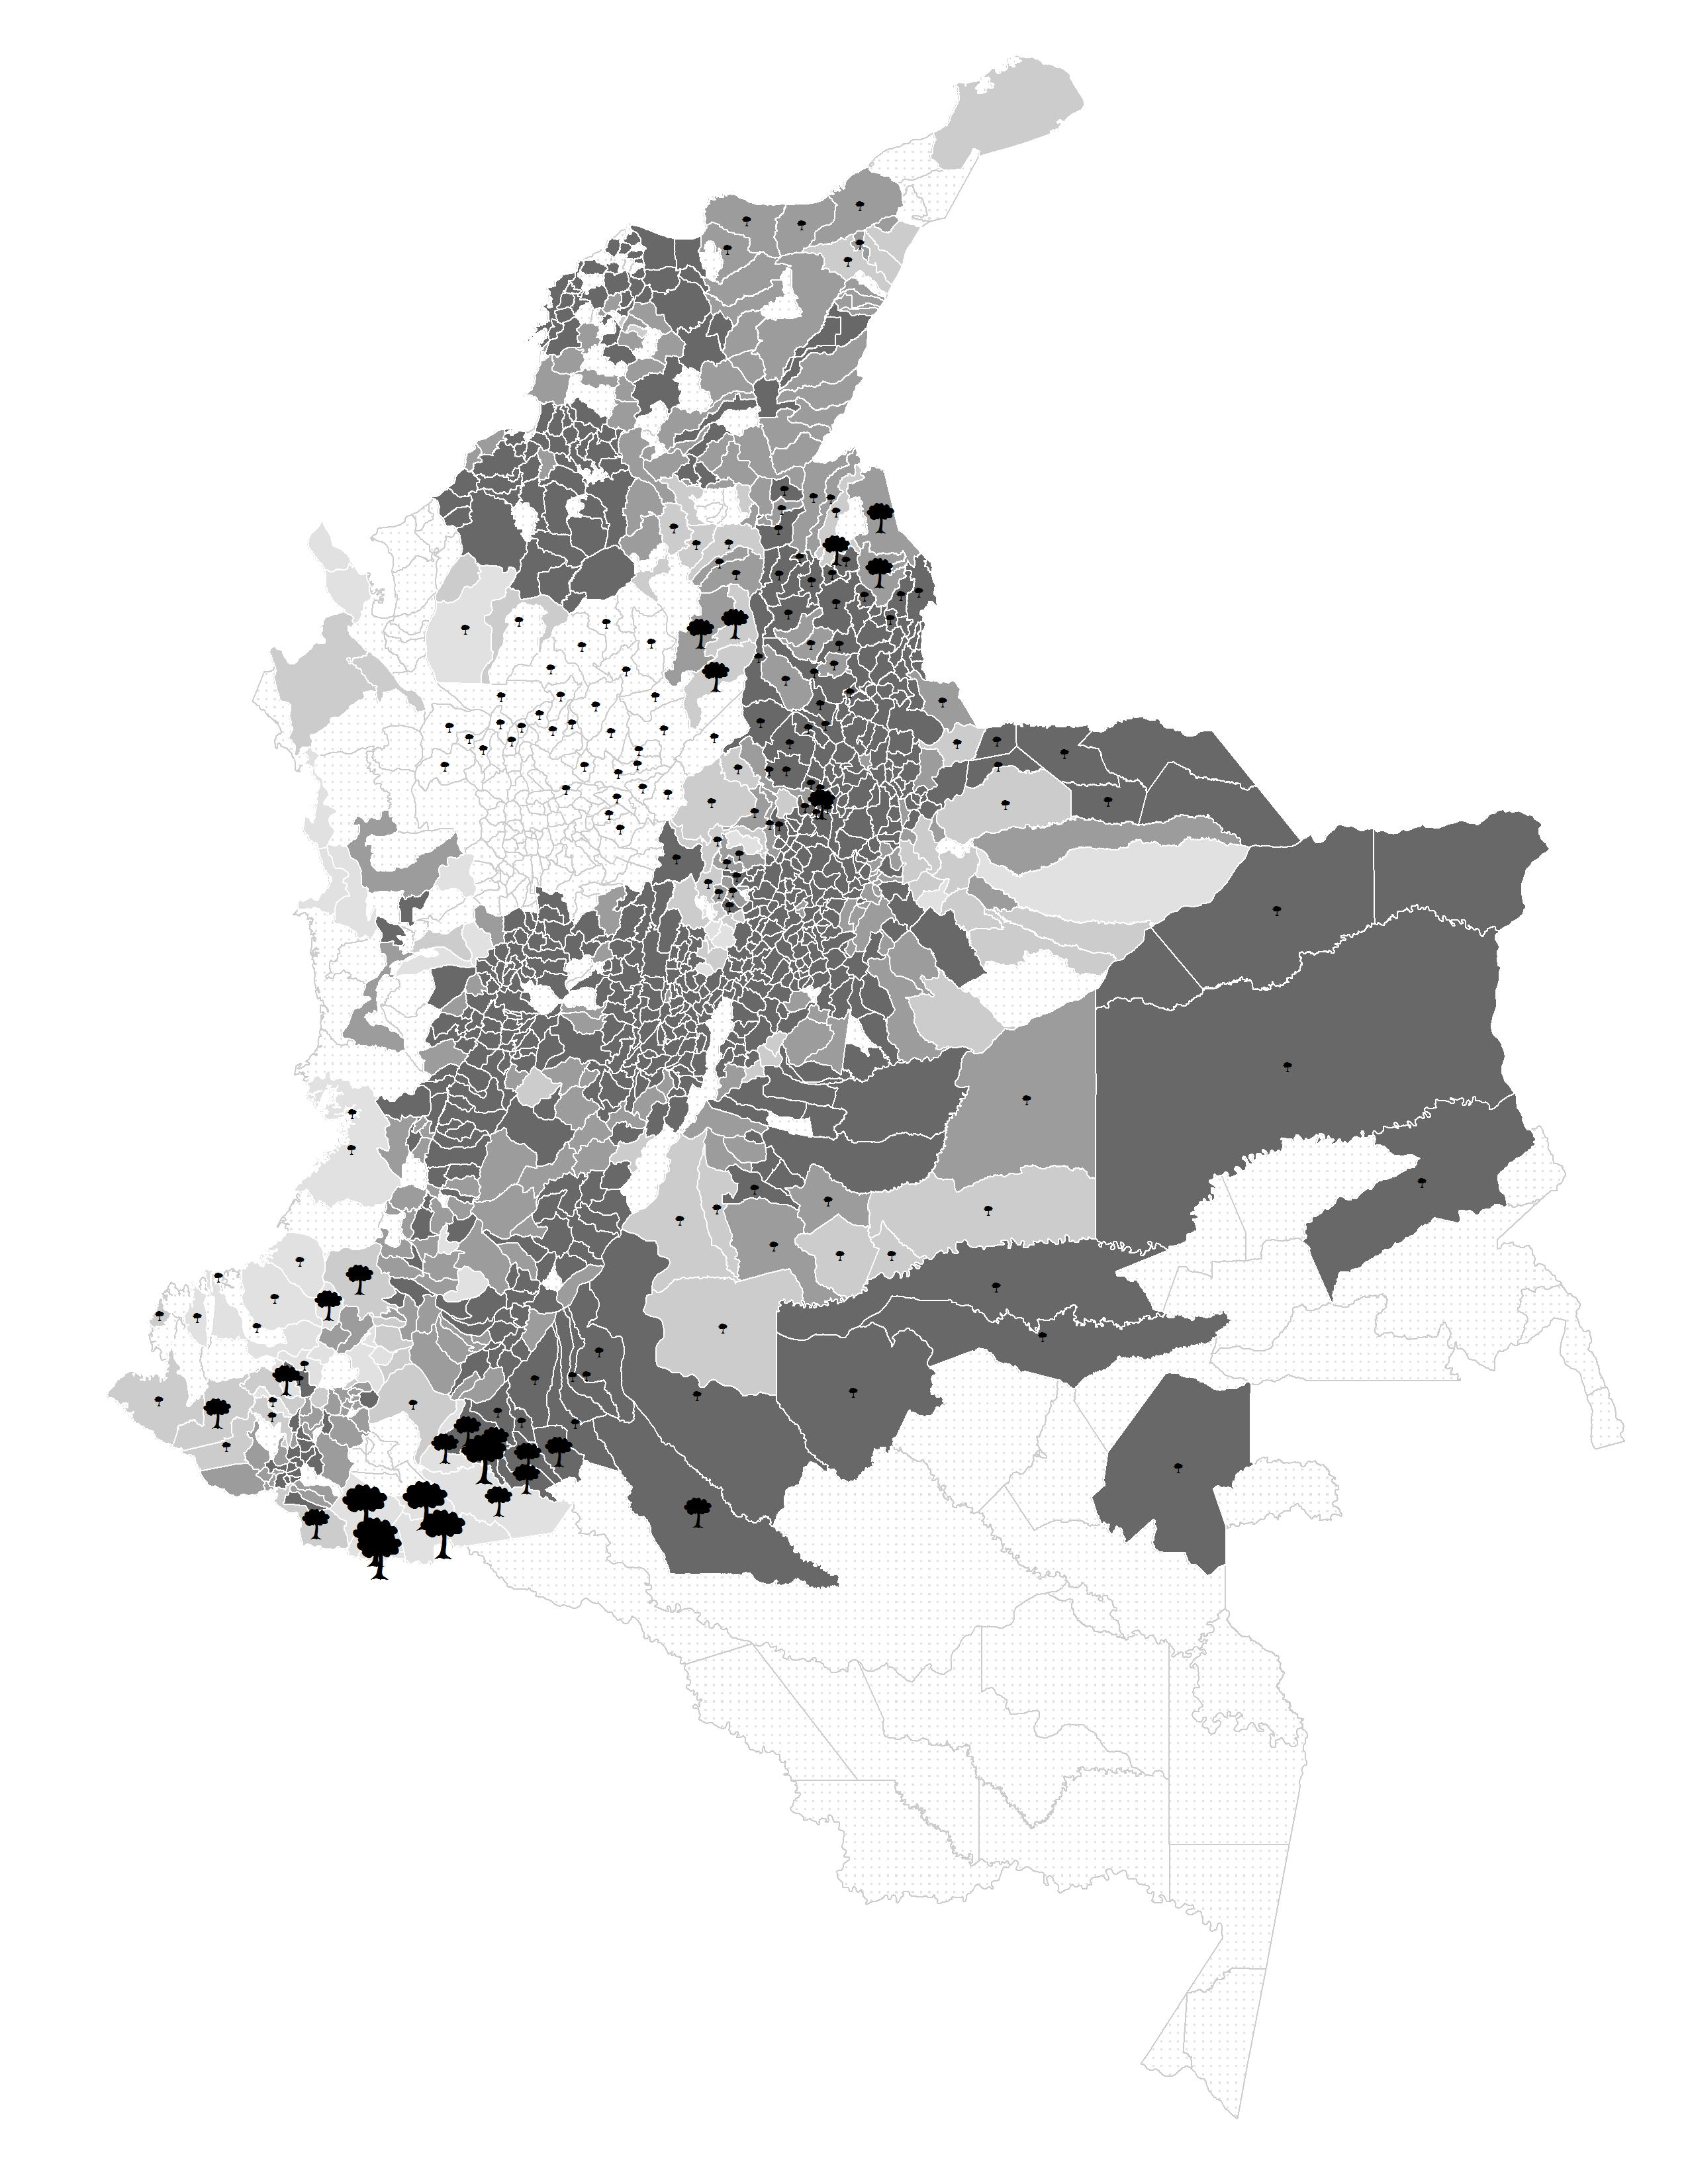
\includegraphics[height=13cm,width=.3\textwidth]{map_1a} & 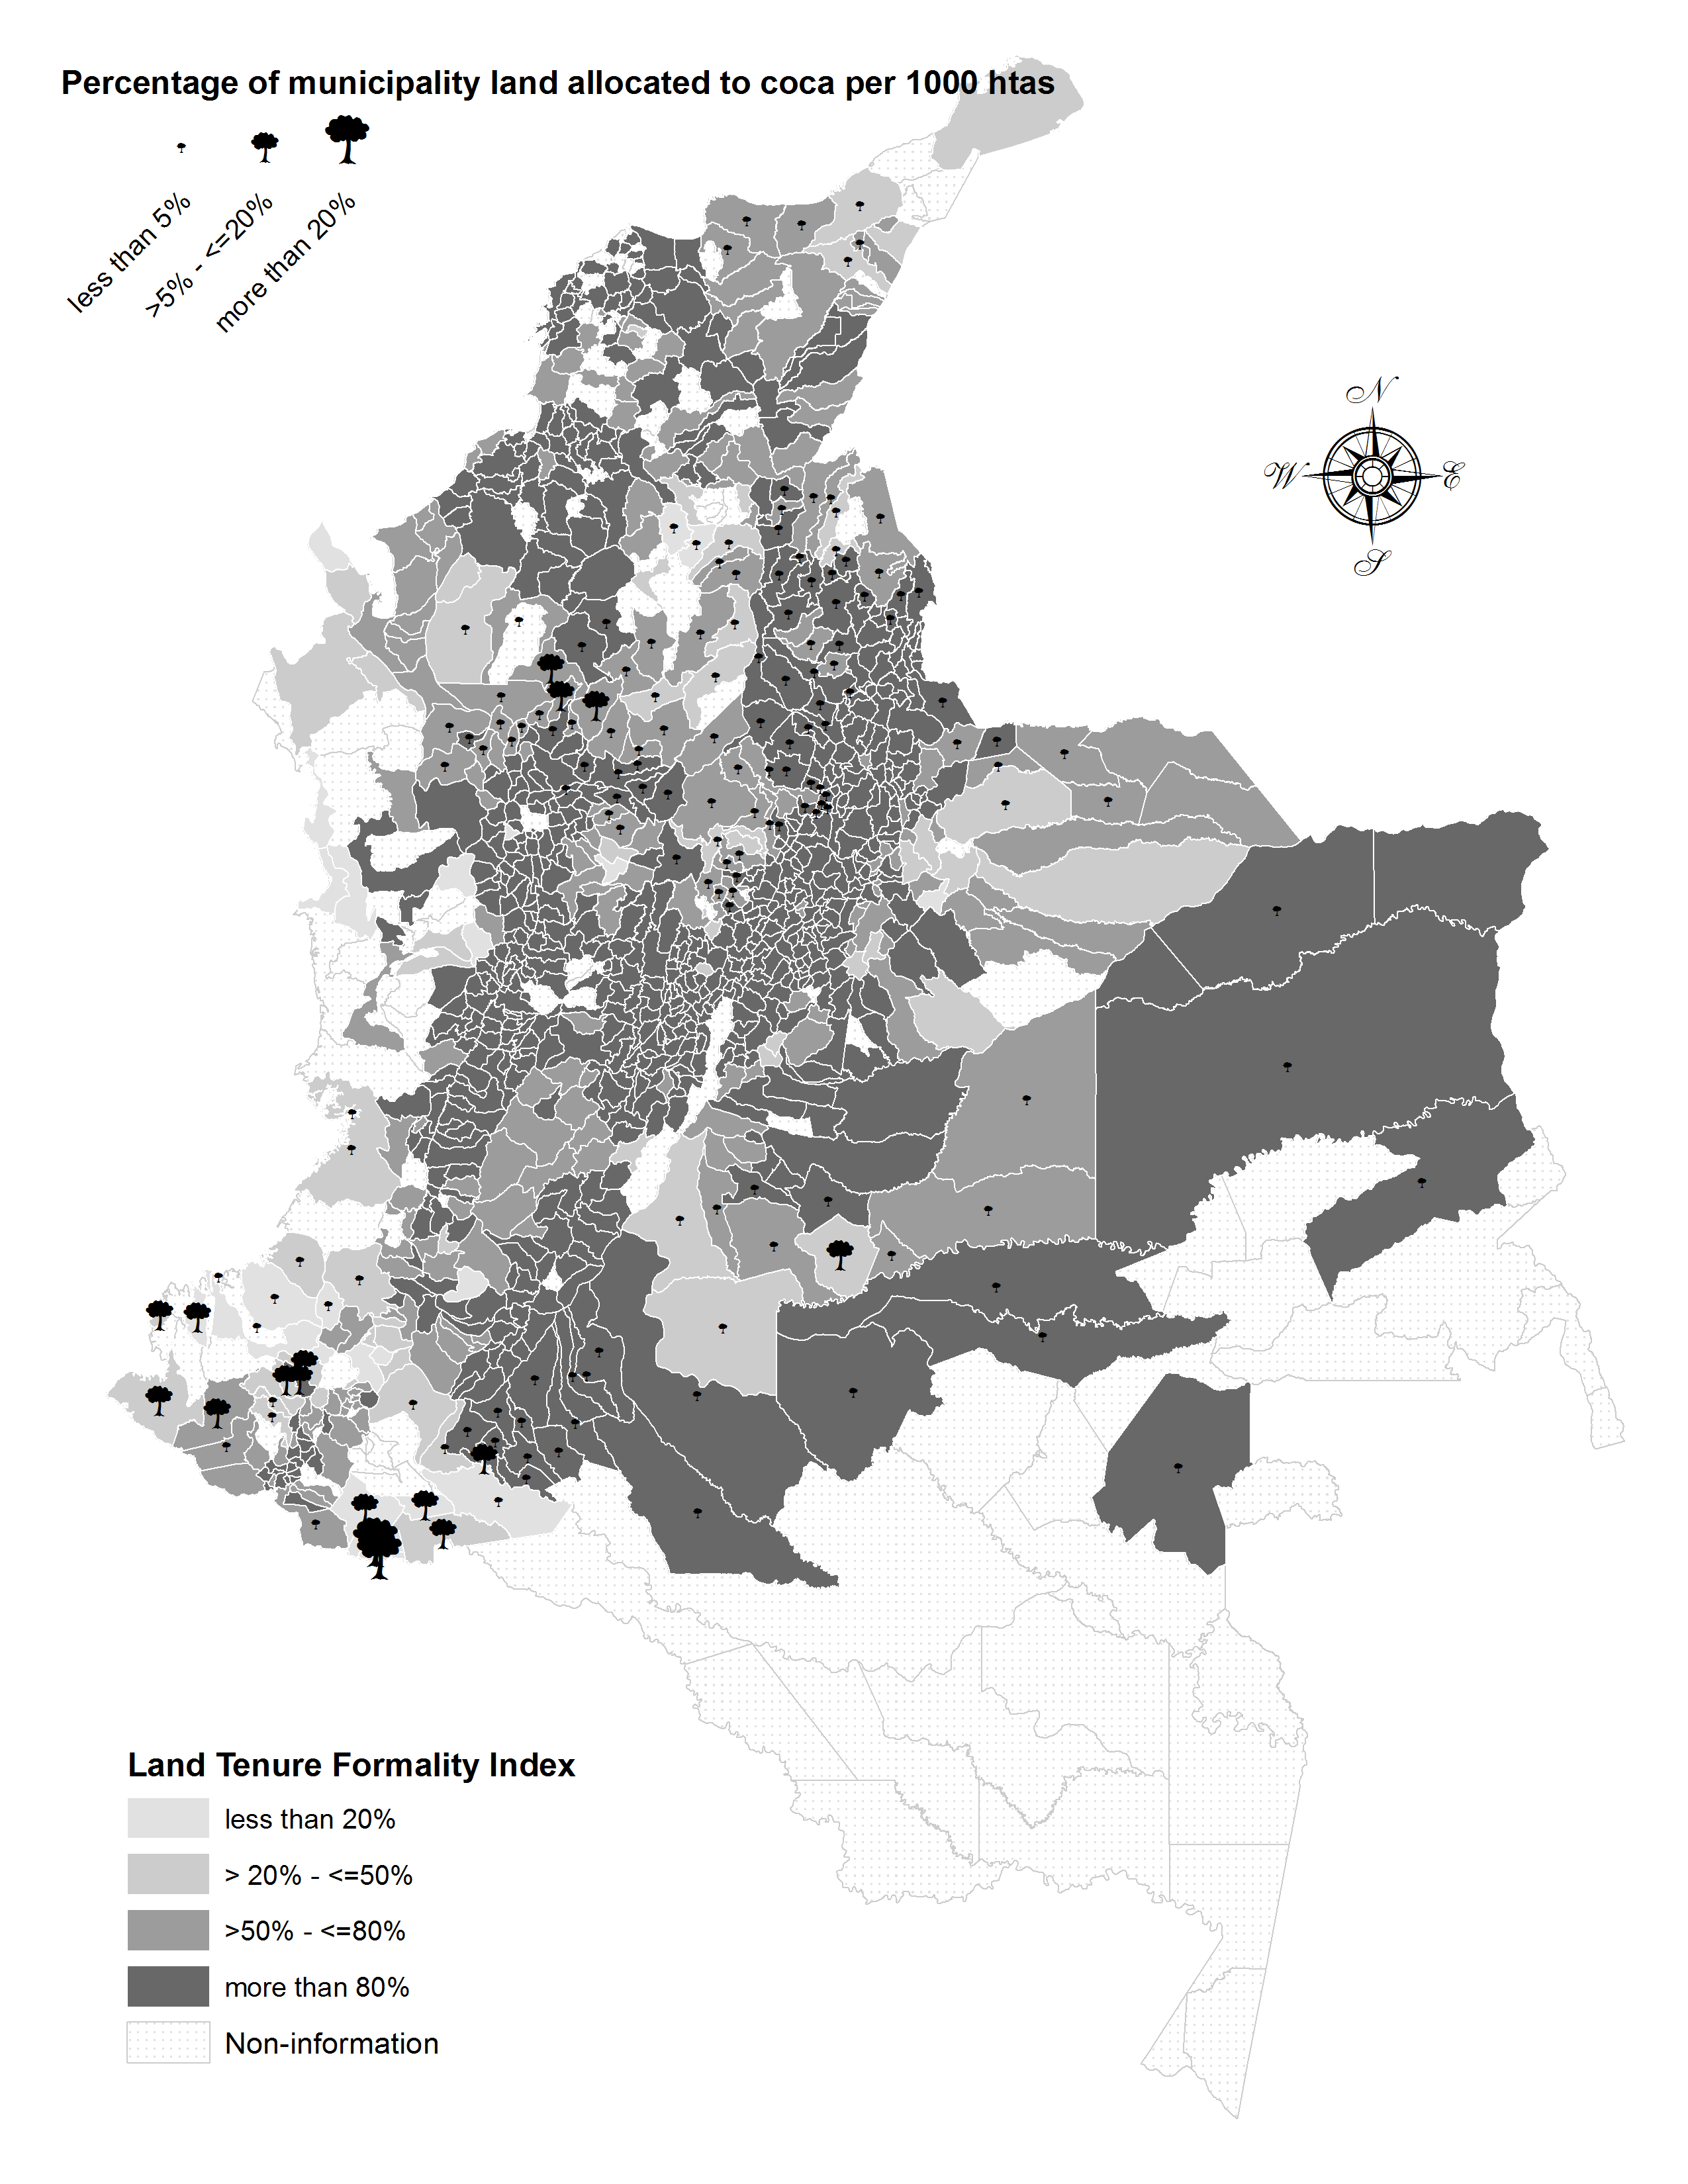
\includegraphics[height=13cm,width=.3\textwidth]{map_1b}   & 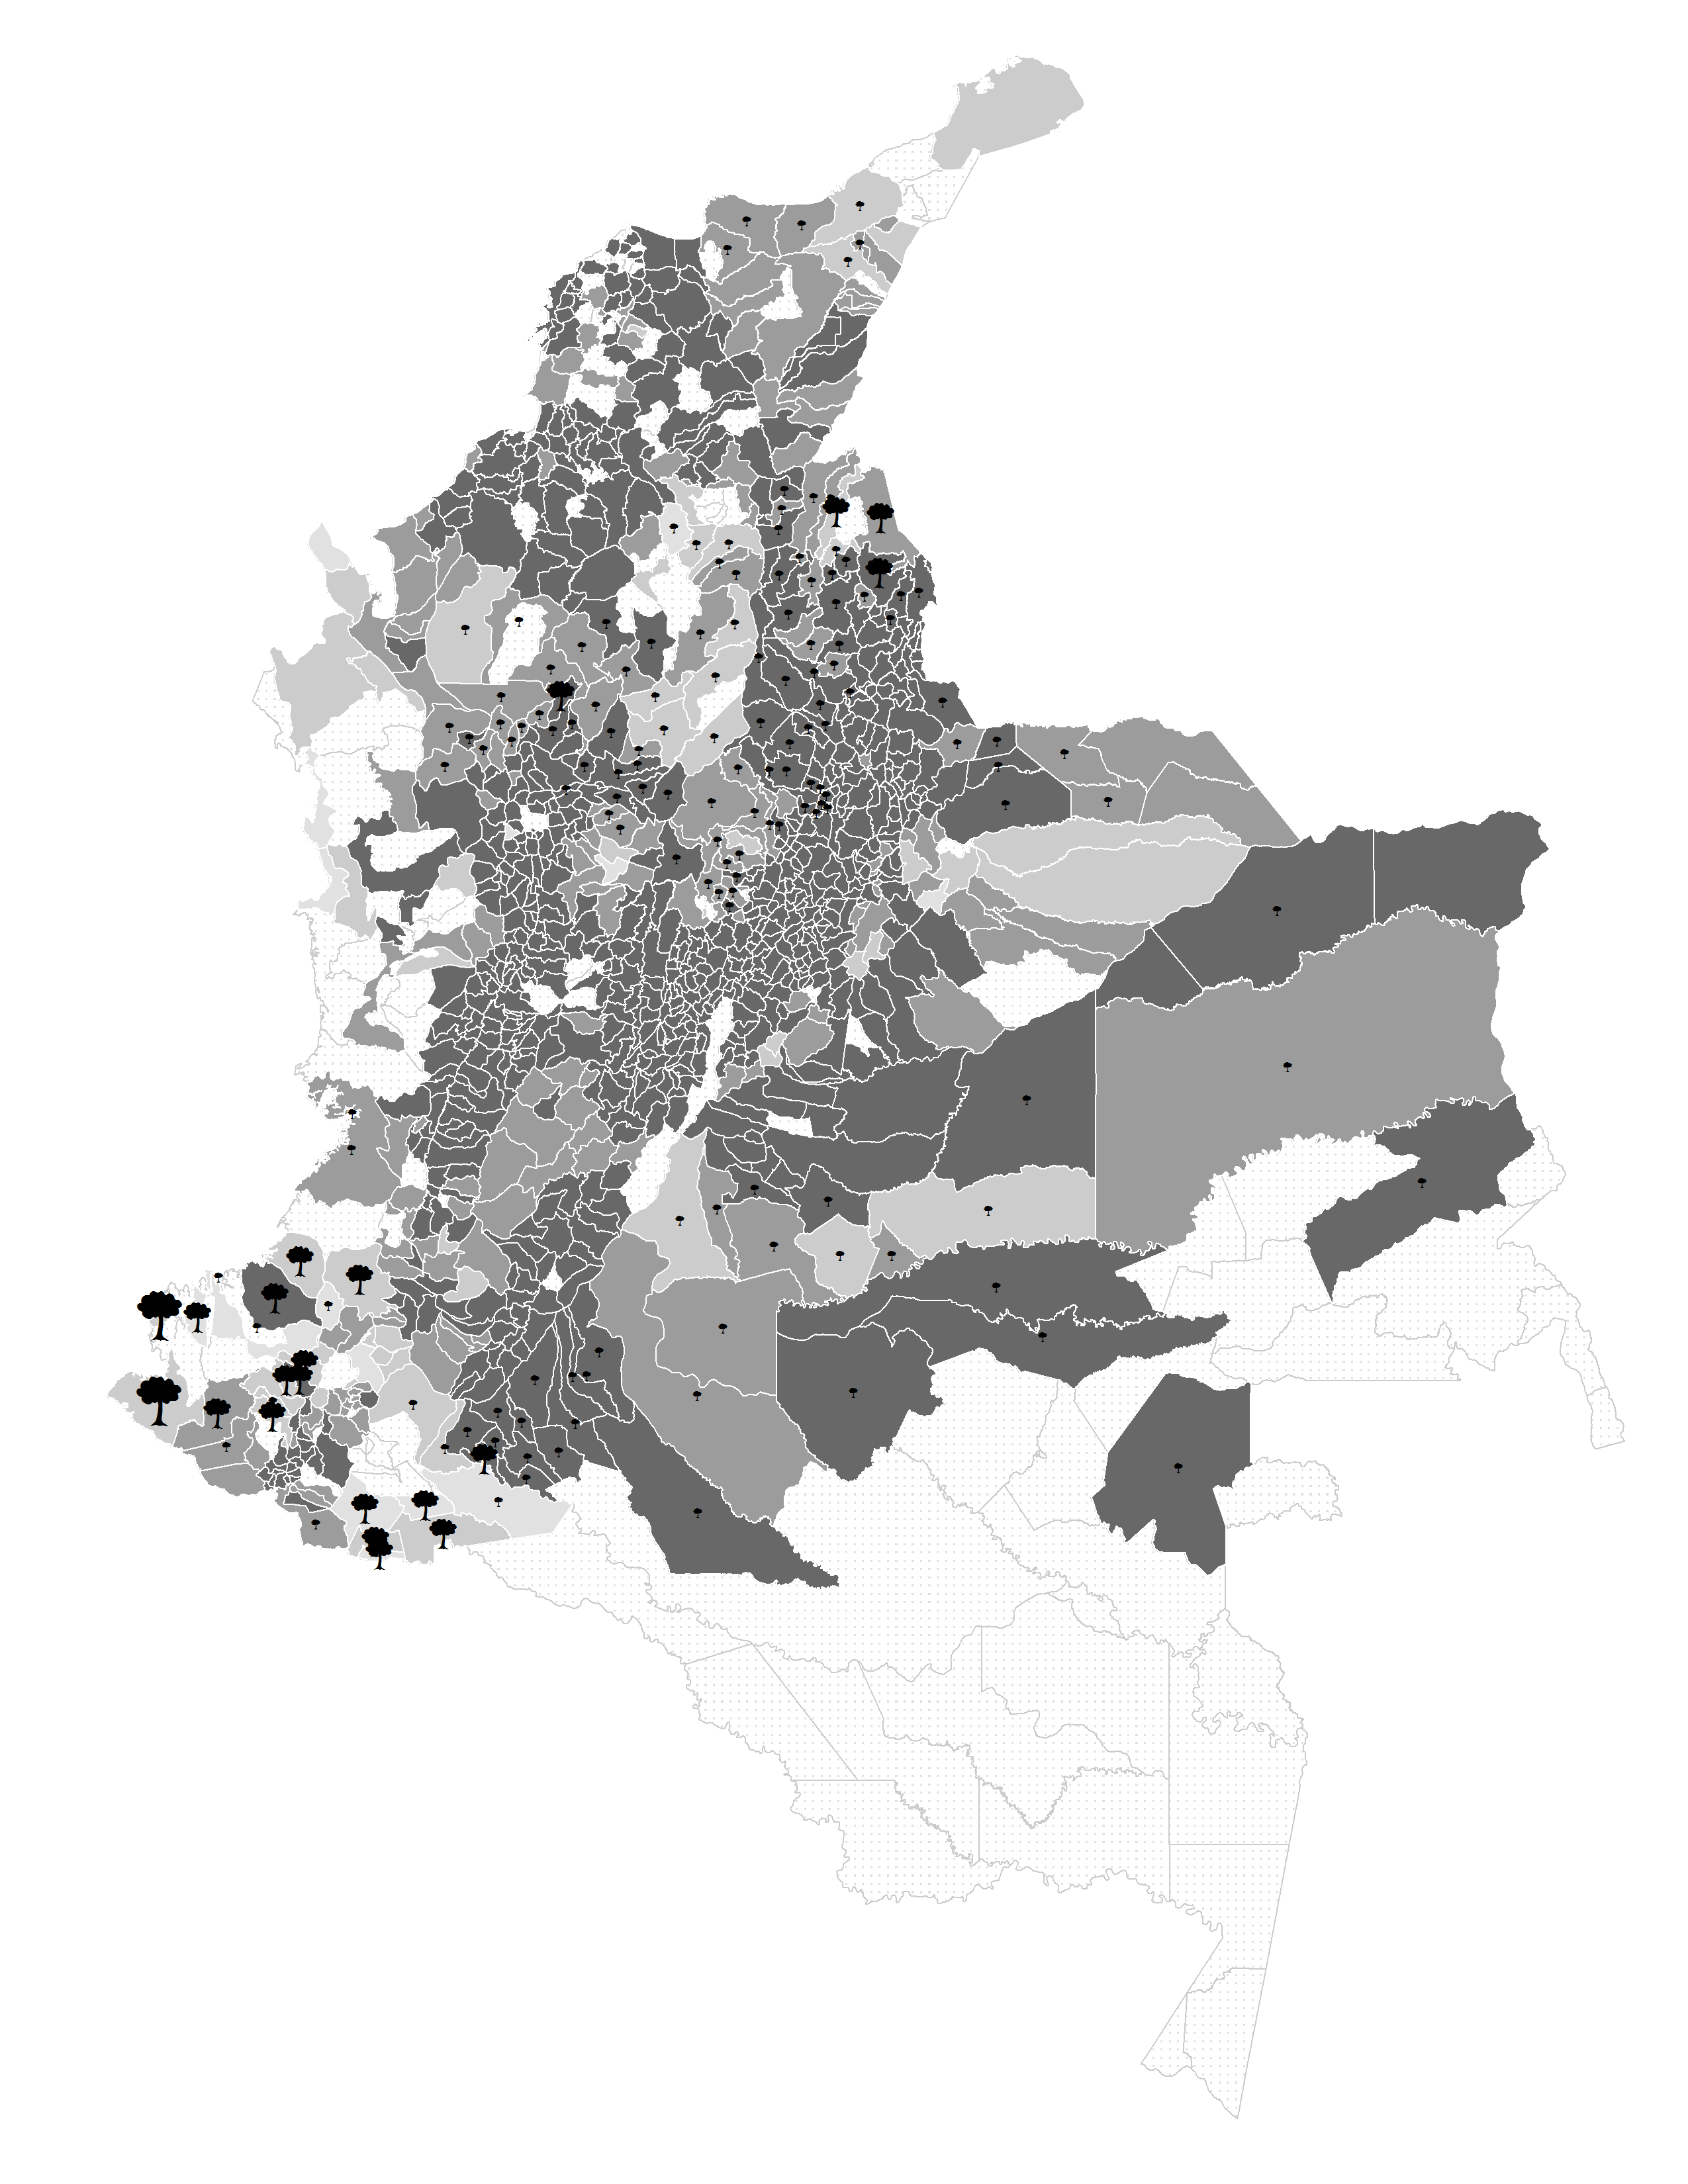
\includegraphics[height=13cm,width=.3\textwidth]{map_1c} \\ 2000 & 2006 & 2009 \\
\multicolumn{3}{p{\textwidth}}{\tiny \emph{Notes -} All maps have the same scale in both variables. In 2000, the department of Antioquia is missing due to information availability. Data source: CEDE, 2013.}
\end{tabular}
\end{figure}
\end{center}
\end{landscape}
\clearpage
 %</mytag>

\end{document}
%%% Graph 3

